\documentclass{llncs}
\usepackage{amssymb}
\usepackage{color}
\usepackage{pgf,pgfarrows,pgfnodes,pgfautomata,pgfheaps,pgfshade}
\usepackage{tikz}
\usetikzlibrary{arrows,decorations.pathmorphing,backgrounds,positioning,fit,petri}
\usepackage{amsmath}

\begin{document}

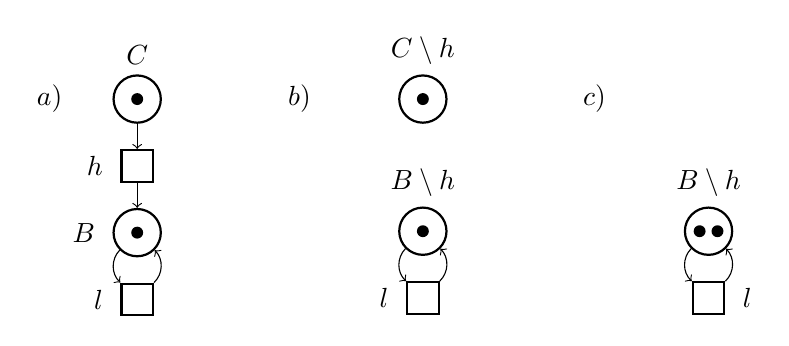
\begin{tikzpicture}[
every place/.style={draw,thick,inner sep=0pt,minimum size=6mm},
every transition/.style={draw,thick,inner sep=0pt,minimum size=4mm},
bend angle=45,
pre/.style={<-,shorten <=1pt,>=stealth,semithick},
post/.style={->,shorten >=1pt,>=stealth,semithick}
]
\def\eofigdist{3cm}
\def\eodist{0.32}
\def\eodisty{0.7}
\def\eodistw{1.05}

\node (a) [label=left:$a)\qquad $]{};

\node (q1) [place,tokens=1] [label={above:$C$} ] {};
\node (t1) [transition] [below=\eodist of q1,label=left:$h\;$] {};
\node (q2) [place,tokens=1] [below=\eodist of t1,label=left:$B\;$] {};
\node (t2) [transition] [below =\eodist of q2,label=left:$l\;$] {};

\draw  [->] (q1) to (t1);
\draw  [->] (t1) to (q2);
\draw  [->, bend right] (q2) to (t2);
\draw  [->, bend right] (t2) to (q2);

% seconda rete

 
\node (b) [right={2.4cm} of a, label=left:$b)\;\;$] {};

\node (p1) [place,tokens=1]  [right=\eofigdist of q1,label=above:$C \setminus h$] {};
\node (p2) [place,tokens=1] [below=\eodistw of p1,label=above:$B \setminus h$] {};
\node (s2) [transition] [below =\eodist of p2,label=left:$l\;$] {};

\draw  [->, bend right] (p2) to (s2);
\draw  [->, bend right] (s2) to (p2);





% terza rete
  
 
\node (c) [right={3.5cm} of b,label=left:$c)\;\;$] {};

\node (r1) [place, tokens=2]  [right=\eofigdist of p2,label=above:$B \setminus h$] {};
\node (v1)  [transition] [below=\eodist of r1,label=right:$\;l$] {};

\draw  [->, bend right] (r1) to (v1);
\draw  [->, bend right] (v1) to (r1);


\end{tikzpicture}

\end{document}